\section{Computation Experiments }
\label{sec:comp_exp}
The experiments are done with Grid5000 \cite{balouek_adding_2012}, " a large-scale and flexible testbed for experiment-driven research in all areas of computer science, with a focus on parallel and distributed computing including Cloud, HPC and Big Data and AI." In specific, the \textit{chuc} cluster, in the Lille center, composed of nodes of 4 GPU A100 with 40G of VRAM was used. 

Apart from aforementioned hyperparameters (learning rate, \acrshort{lora} rank ... ) and configuration (weight matrix to apply \acrshort{lora}), all arguments of LitGPT CLI is used with default value. The only exception is the number of epochs, fixed to 1 to reduce computation costs. For next sections, a difference will be made between variables (value inside optimization range), and hyperparameters (value used by the training function) to clarify the reading of the value. 

Using this configuration, one epoch of fine-tuning is taking around 31 minutes. For the evaluation on both datasets, it's taking around 12 minutes. Based on previous articles, and evaluations durations, the total evaluation budget for experiments is 50 evaluations by each algorithms, including a sampling budget of 10 for \acrlong{bo}. 

The implementation of the previous algorithm, the objective function and next experiments are all stored in github, following this link : \url{https://github.com/Kiwy3/BO_PBO_HPO_LLM}.

%%%%%%%%%%%%%%%%%%%% Sampling Experiment %%%%%%%%%%%%%%%%%%%%%%%%%%
\subsection{Sampling experiment}
\label{sec:samp_exp}

For the sampling experiment, \acrfull{lhs} was used with the same budget as other, i.e. 50 evaluations. Whole experiments took 36 hours. The aims of this experiments is dual: first, make a lower bound reference for others experiments, and second, explore the search space and the score behavior. To use as a lower bound, \acrshort{lhs} achieve scores of 37.6\% for MMLU, and 47.9\% for Hellaswag. Theses score are inside table \ref{tab:bounds}.

\begin{figure}
    \centering
    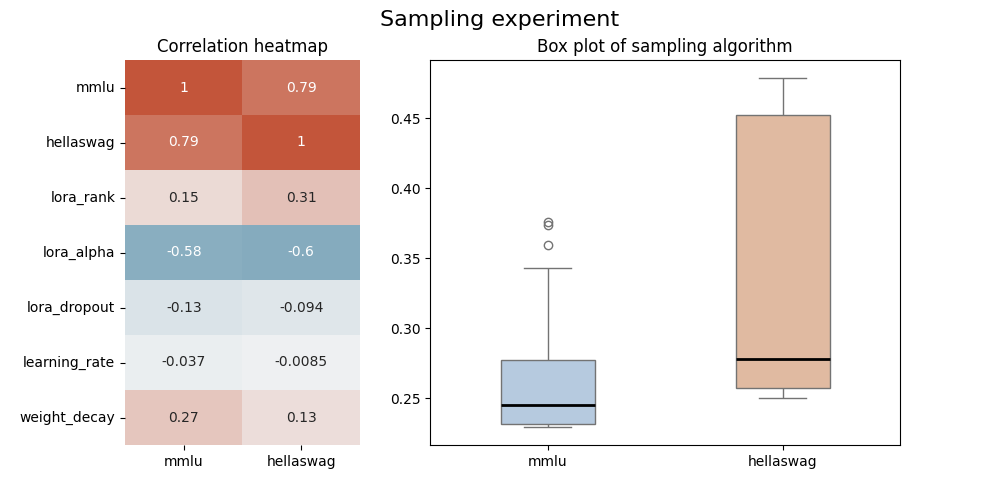
\includegraphics[width=0.6\linewidth]{figures/sampling/lhs.png}
    \caption{results of \acrlong{lhs} experiment}
    \label{fig:lhs_exp}
\end{figure}

The correlation between MMLU and Hellswag tend to confirm the relevance of their choice as a pair for validation and testing dataset. It's sufficiently high to guess that most of \textit{good} model for one will be good for the other one, but it's still less than one, making over-fitting visible if present.

For variables, it look like LoRA alpha, the scaling parameter of LoRA, is the most influent on the score, be it Hellaswag or MMLU. Next to it, LoRA Rank and weight decay are the most influent, with a difference in ranking on the metrics. With this first exploration, it look like Dropout and Learning rate are not very effectful for this problem, be it the choice of their range or the implementation. 

On the distribution of the score values, it's interesting to note that Hellaswag has a broader range of score, making it useful for efficiently discriminating solutions.  With a broader thinking, the sampling experiment confirm the relevance to apply \acrshort{hpo} algorithms to the described problem. If scores were independent from variables, or all scores were the same, \acrshort{hpo} would be useless. 

%%%%%%%%%%%%%%%%%%%% BO Experiment %%%%%%%%%%%%%%%%%%%%%%%%%%
\subsection{\acrshort{bogp} experiment}
\label{sec:bo_exp}
Figure \ref{fig:bo_res} depicts the performance of \acrfull{bogp} over 50 iterations, measured in terms of the \Gls{hs} accuracy. This visualization highlights the evolution of the optimization process as it transitions from sampling to the exploitation, and ultimately converges towards high-performing solutions.


\begin{figure}[h!]
    \centering
    \begin{subfigure}[b]{.50\textwidth}
      \centering
      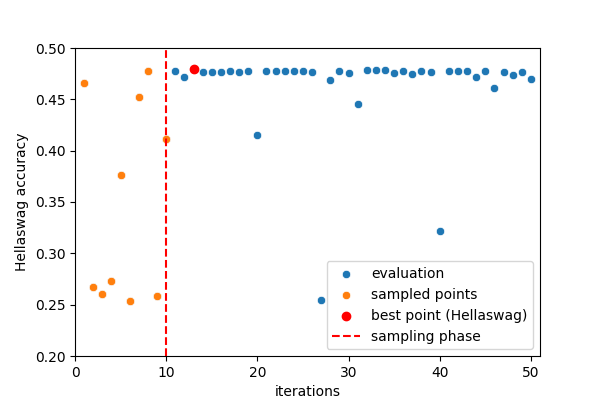
\includegraphics[width = \textwidth]{figures/bo/score_evolution.png}
      \caption{Score over time}
      \label{fig:bo_score_time}
    \end{subfigure}%
    \begin{subfigure}[b]{.40\textwidth}
      \centering
      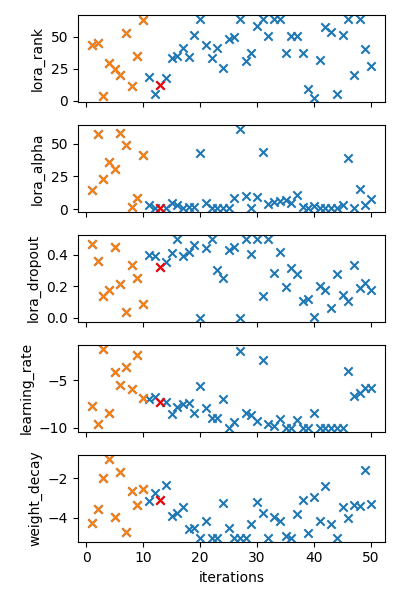
\includegraphics[width = 0.6\textwidth]{figures/bo/variables_evolution.png}
      \caption{Variable over time}
      \label{fig:bo_var_time}
    \end{subfigure}
    \caption{Experiment using \acrshort{bo} algorithm}
    \label{fig:bo_res}
\end{figure}

During the sampling phase, as shown by figure \ref{fig:bo_score_time}, evaluated solutions have the same diversity of solutions than the full sampling experiment, allowing to efficiently extract knowledge from the search space. The algorithm achieve a stable convergence to mostly high-performing solution.

If we briefly look at figure \ref{fig:bo_var_time}, it's interesting to look at the diversity of configuration to obtain high-performance, and the trend of the algorithms for each variables. For example, for LoRA alpha, or learning rate, we can observe a clear trend toward the lower bound of the optimization range. 

To summarize, this experiment demonstrate the effectiveness of Bayesian Optimization in efficiently exploiting the knowledge of the search space obtained in the sampling phase. The optimization process still explore area with high uncertainty, giving few low-performing solution.


%%%%%%%%%%%%%%%%%%%% SOO Experiment %%%%%%%%%%%%%%%%%%%%%%%%%%
\subsection{\acrshort{soo} experiment}
\label{sec:soo_exp}

On this experiment, we observe in Figure \ref{fig:soo_res} the behavior of \acrshort{soo} as it optimizes the given objective function. The figure illustrates how the algorithm navigates the search space, iteratively improving the solution by adjusting the hyperparameters. By examining the trends in performance metrics and variables evolution, we aim to analyze the convergence behavior, stability, and overall effectiveness of \acrshort{soo} in this setting.

\begin{figure}[h!]
    \centering
    \begin{subfigure}[b]{.5\textwidth}
      \centering
      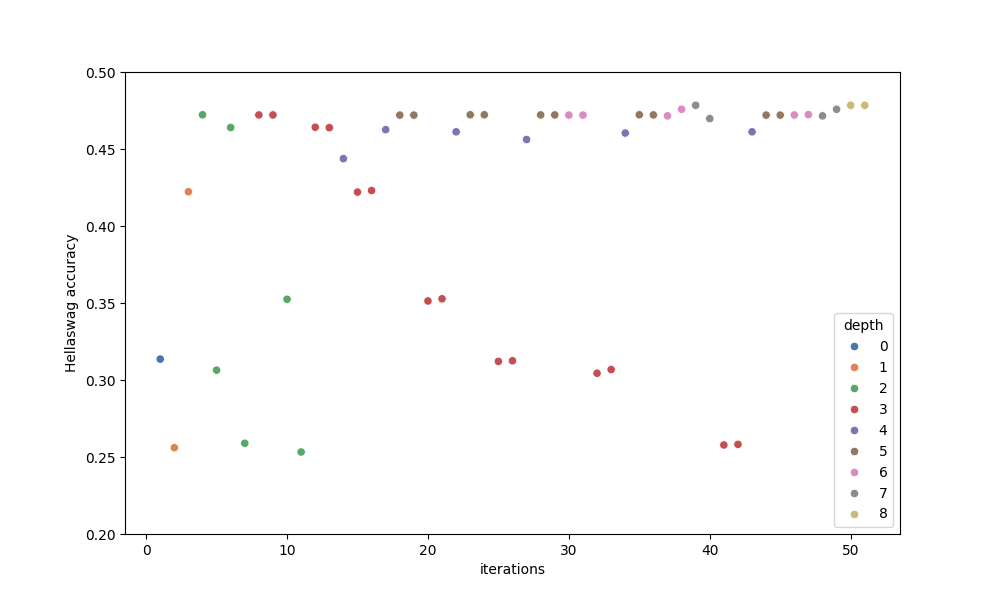
\includegraphics[width = \textwidth]{figures/soo/score_evolution.png}
      \caption{Score over time}
      \label{fig:soo_score_time}
    \end{subfigure}%
    \begin{subfigure}[b]{.4\textwidth}
      \centering
      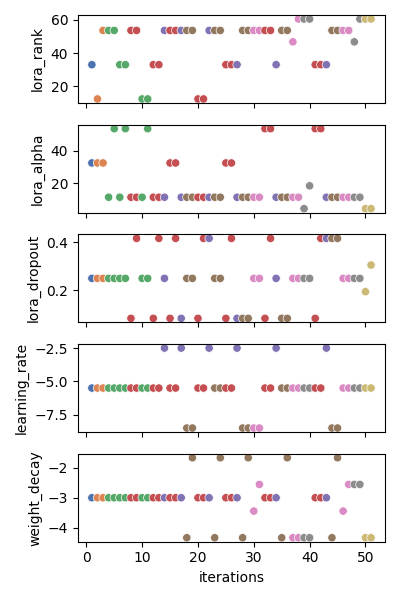
\includegraphics[width = 0.5\textwidth]{figures/soo/variables_evolution.png}
      \caption{Variable values over time}
      \label{fig:soo_var_time}
    \end{subfigure}
    \caption{Experiment using \acrshort{soo} algorithm}
    \label{fig:soo_res}
\end{figure}


Figure \ref{fig:soo_score_time} depicts the accuracy of the \gls{hs} dataset as a function of iterations, with marker colors representing different depth configurations. The observed trend suggests that most configurations achieve accuracies arround 0.46 throughout the optimization process. Several configurations converge toward the higher end of this range, indicating potential stability and effectiveness in learning as iterations progress. 

It is evident that higher-depth configurations tend to cluster around higher accuracy values, while lower depths display more scattered behavior across the accuracy spectrum. In specific, depth 2, with a section on lora alpha seems to greatly affect the performance on the accuracy. On figure \ref{fig:soo_var_time}, it's clear on the limitation of constrained-budget \acrshort{soo} without local exploitation at the end of the algorithms : Only a few number of values by variables are explored : around 5 by variables, making it equivalent to exploration of a search space of $6^5=7,776$ discrete solutions.

To summarize, \acrshort{soo} achieve a maximum performance closed to the precedent algorithm, but explore a restricted number of configuration, and lose time by evaluating unpromising solutions.
%%%%%%%%%%%%%%%%%%%% BaMSOO Experiment %%%%%%%%%%%%%%%%%%%%%%%%%%
\subsection{\acrshort{bamsoo} experiment}
\label{sec:bamsoo_exp}

The last experiment of this work is using \acrshort{bamsoo}, with $\eta = 1$ in equation \ref{eq:ucb}, to reduce the confidence interval and promote approximation, to avoid the evaluation of unpromising points. To look after it, figure \ref{fig:bamsoo_score_time} discriminate evaluated and approximated points, and might be compared with \ref{fig:soo_score_time} to look after approximated points.



\begin{figure}[h]
    \centering
    \begin{subfigure}[b]{.5\textwidth}
      \centering
      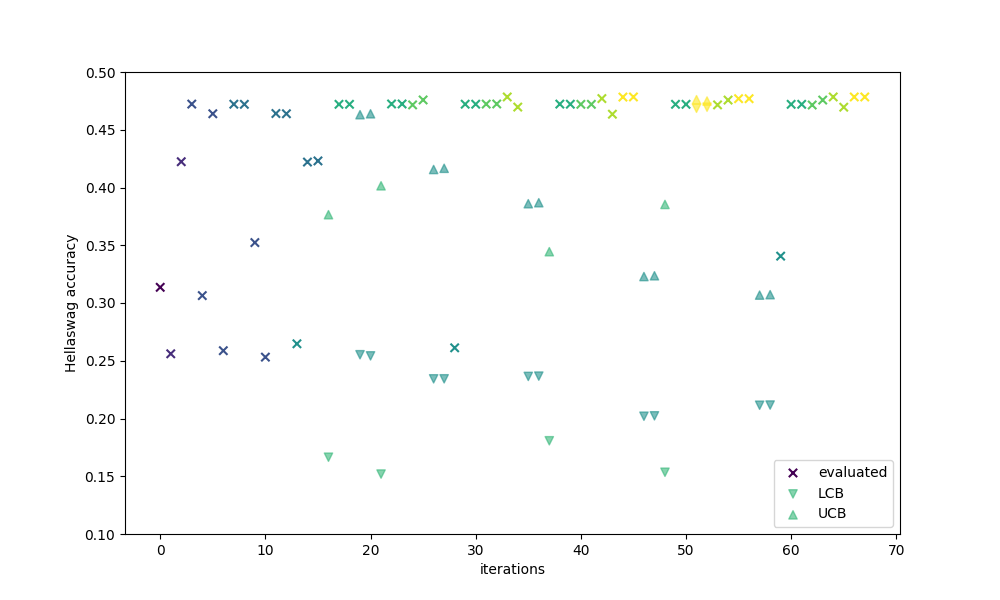
\includegraphics[width = 0.9\textwidth]{figures/bamsoo/score_evolution.png} 
      \caption{Score over time}
      \label{fig:bamsoo_score_time}
    \end{subfigure}%
    \begin{subfigure}[b]{.4\textwidth}
      \centering
      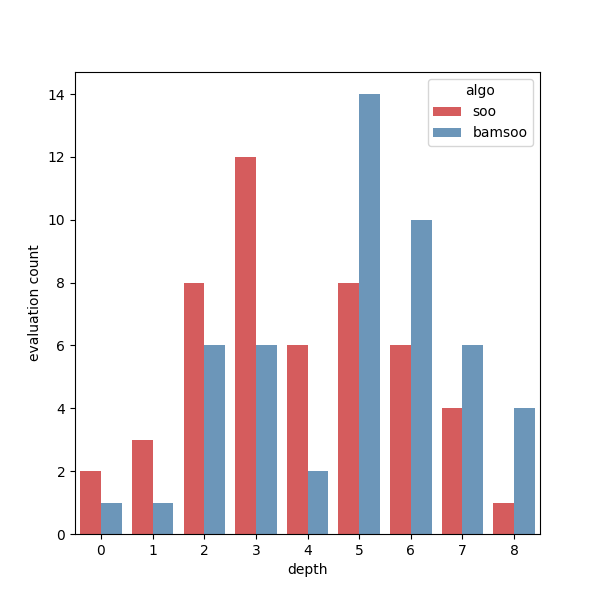
\includegraphics[width = 0.7\textwidth]{figures/bamsoo/depth_compar.png} 
      \caption{Depth exploration }
      \label{fig:bamsoo_soo_depth}
    \end{subfigure}
    \caption{Experiment using \acrshort{bamsoo} algorithm}
    \label{fig:bamsoo_res}
\end{figure}

When compared to figure \ref{fig:soo_score_time}, the pair of evaluations for depth 2, with low-performing solutions seems to have mostly been approximated. On the whole experiment, 16 points were approximated, to efficiently search further than \acrshort{soo}. Figure \ref{fig:bamsoo_soo_depth} compare the budget allowed on each depth, and highlight the focus of \acrshort{bamsoo} for lower depth exploration.
To summarize, \acrshort{bamsoo} achieve to speed up \acrshort{soo}, but is still slow in comparison with \acrshort{bo} at first glance. Moreover, \acrshort{bamsoo} succeed to prevent most of low-performing evaluation of \acrshort{soo}.








%%%%%%%%%%%%%%%%%%%% Analysis %%%%%%%%%%%%%%%%%%%%%%%%%%

\subsection{Comparison and Analysis}
\label{sec:comparison}

To conclude this section, it's crucial to directly compare algorithms, especially their performance, with validation and testing dataset. To look at absolute performance, and not only relative between algorithms, lower and upper bounds will be used. 

\begin{table}[h!]
    \centering
    \begin{tabular}{|c||c|c||c|c|c|}
    \hline
       Datasets  & Lower (LHS) & Upper (model card) & BO-GP & SOO & BaMSOO \\
    \hline
       Hellaswag (validation)  & 47.90 & 41.5 & 47.91 & 47.84 & 47.84\\
       MMLU (testing) & 37.61 & 49.3 & 38.11 & 37.42 & 37.50 \\
    \hline
    \end{tabular}
    \caption{Bounds on accuracy for validation and testing dataset}
    \label{tab:bounds}
\end{table}
In face of such experiments, it's interesting to look at bounds of the metric, to compare the results. The lower bounds is the results of the experiment using solely \acrshort{lhs} to pick solutions, with the same number of evaluation than algorithms. \acrshort{lhs} being intrinsically parallel, if evaluated algorithms don't achieve better performance than a solely exploring one, their benefit isn't relevant. 

For the higher bound, I will look at the higher value in the model card\footnote{\url{https://huggingface.co/meta-llama/Llama-3.2-1B}} of the model, achieved using advanced fine-tuning methods like Supervised Fine-Tuning (SFT), Rejection Sampling (RS), and Direct Preference Optimization (DPO). Values are inside table \ref{tab:bounds}.

\begin{figure}[h]
    \centering
    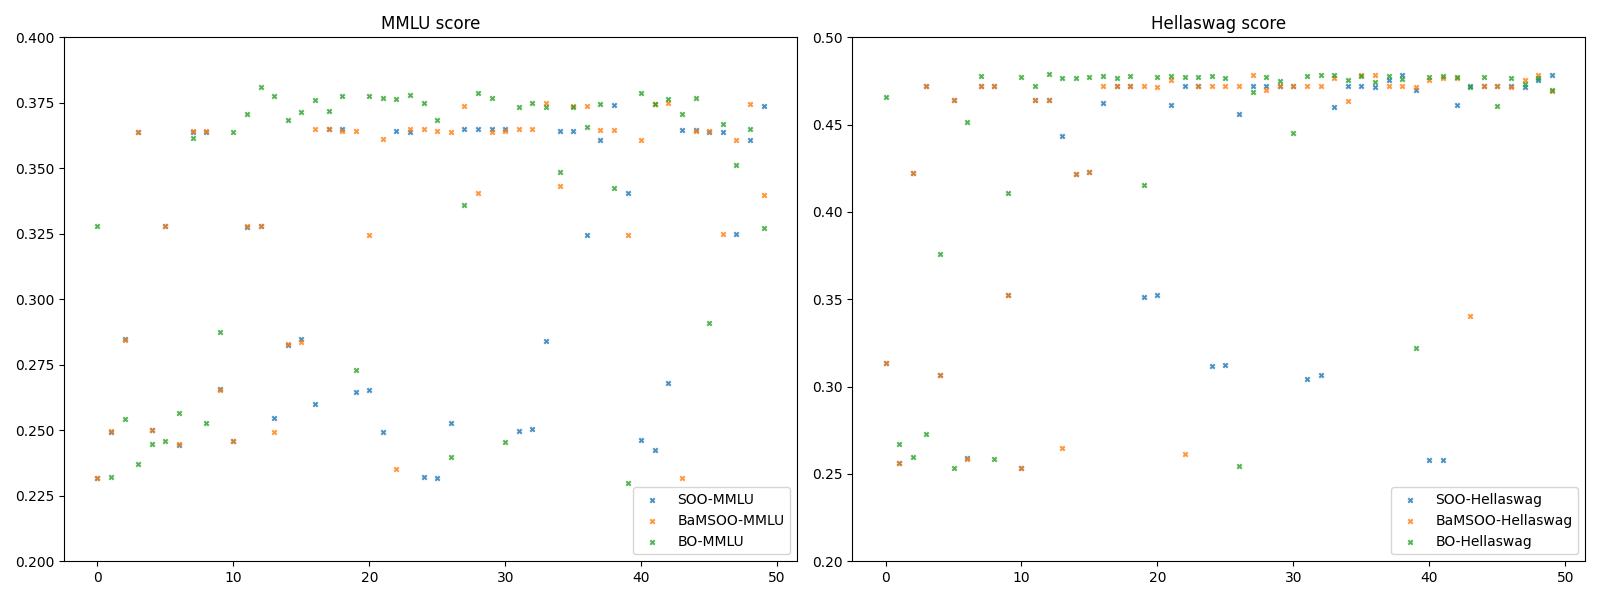
\includegraphics[width=0.8\textwidth]{figures/global/comparison.png}
    \caption{Comparison between 3 algorithms on 2 metrics}
    \label{fig:global_compare}
\end{figure}


At first, what's interesting is to look at testing and upper bounds results. Since the upper bound is mostly fine-tuned with aimed for MMLU results, the \Gls{hs} upper bounds isn't really relevant. Considering this, the analysis of this part will mostly be done with MMLU. The best results with MMLU is \acrfull{bo}, being 23\% from the upper bound.




With figure \ref{fig:global_compare}, it's clear than \acrshort{bo} algorithm is a step more performing than others algorithms for this problem, especially with the low number of low-performing solutions evaluated. Apart from this part, the whole results may suggest that the objective function, or the search space could be different, to have an higher range of results for comparison. 










